\section{Probability Analysis}
\label{ch:probability}

Open from `3.\ Analysis $\to$ Probability Analysis`.

Reynolds stresses, spectra, and correlations all describe the flow through low-order moments. Two flows can share the same mean and the same variance and still behave very differently: one may fluctuate gently about the mean, the other may sit quiet most of the time and burst violently at rare instants. Recovering that information requires the full probability distribution of the fluctuations rather than its first two moments. This chapter covers the four diagnostics grouped in the `Probability Analysis` window, each in its own tab:

\begin{itemize}[leftmargin=1.5em]
  \item \textbf{PDF}: histograms of the instantaneous velocity components and their fluctuations, with skewness and flatness.
  \item \textbf{Flow Direction}: maps of forward-flow and reverse-flow probability, used to locate and quantify separation.
  \item \textbf{Binary Space-Time}: the sign of the fluctuation along a line plotted against time, revealing the passage of coherent structures (TR only).
  \item \textbf{Quadrant}: decomposition of the Reynolds shear stress into ejections, sweeps, and interactions.
\end{itemize}

\begin{quote}
\textbf{Note:}
All four tabs count valid samples \emph{per grid point}. Masked or invalid vectors (NaN) are excluded from the sample count at that point rather than being treated as zeros, so a point with $k$ valid snapshots out of $N$ is normalised by $k$, not by $N$. A point with no valid samples returns NaN and is rendered as background, not as a probability of zero. Points whose valid-sample count is very low still produce a number, so check the sample-count readout before interpreting isolated extreme values.
\end{quote}

\subsection{PDF tab}

The probability density function $p(q)$ of a quantity $q$ is estimated as a normalised histogram, so that
\[
\int_{-\infty}^{\infty} p(q)\,\mathrm{d}q = 1 ,
\]
that is, the bar heights are divided by both the total number of valid samples and the bin width. Densities from different datasets, different sample counts, and different bin settings are therefore directly comparable. Selecting `Counts` instead of `Density` shows raw bin counts, which is convenient for reading off sample numbers but is not comparable across datasets.

Available quantities are the instantaneous components $u$, $v$, $w$ and the magnitude $|\mathbf{V}|$, and the fluctuations $u' = u - \langle u \rangle$, $v' = v - \langle v \rangle$, $w' = w - \langle w \rangle$, where $\langle \cdot \rangle$ denotes the ensemble average over snapshots at each grid point. The $w$ and $w'$ options are available for stereo (2D3C) data only.

Two shape measures are reported alongside each histogram:
\[
S = \frac{\langle q'^3 \rangle}{\langle q'^2 \rangle^{3/2}}, \qquad
F = \frac{\langle q'^4 \rangle}{\langle q'^2 \rangle^{2}} .
\]
The skewness $S$ measures asymmetry: $S = 0$ for a symmetric distribution, $S < 0$ when large negative excursions dominate. The flatness (kurtosis) $F$ measures the weight of the tails, with $F = 3$ for a Gaussian. Values well above 3 indicate intermittency, that is, rare events far stronger than the r.m.s. level, which is the classical signature of small-scale turbulence. Values well below 3 indicate the opposite: a flat-topped or bimodal distribution, which is what you get when the sampling region spans two distinct flow states rather than one turbulent field. Both are reported in the status bar below the plot, alongside $N$, the mean, the standard deviation, and the sample minimum and maximum.

\subsubsection*{Sampling modes}

\begin{itemize}[leftmargin=1.5em]
  \item \textbf{Point}: click a grid point on the field. The PDF is built from the $N_t$ snapshots at that point only.
  \item \textbf{Line}: select `Horizontal` or `Vertical`, then either drag the line on the preview or type the endpoints into the `Line Entry` boxes ($x_0$, $y_0$, $x_1$, $y_1$) and click `Set line`, exactly as in the Reynolds Stress and TKE Budget modules. All grid points on the line and all snapshots are pooled into one distribution; the plot title reports how many points the line covers. Free (arbitrary-angle) lines are deliberately not offered here, because pooling points sampled by interpolation along an oblique line mixes interpolated values into the statistics.
  \item \textbf{ROI}: drag a rectangle. All points inside it are pooled across all snapshots.
  \item \textbf{Whole field}: every valid point in the domain, across all snapshots.
\end{itemize}

\subsubsection*{Histogram controls}

The number of bins is user-set. As a rough guide, aim for at least a few hundred samples per bin in the core of the distribution; a point-mode PDF from 200 snapshots supports perhaps 15 to 20 bins, whereas a whole-field PDF from the same dataset easily supports 100.

The bin range is set either manually through the `min` and `max` boxes or automatically by ticking `Auto (robust) range`, which clips the range to robust percentiles so that a handful of outliers cannot stretch the axis and collapse the entire distribution into one or two bins. Fixing the range manually is the right choice when comparing several cases, since identical bin edges are required for the histograms to be superimposable. `Gaussian overlay` draws a normal distribution with the same mean and standard deviation as the data, which is the quickest visual test of normality. `Log y` switches the density axis to logarithmic, making the tails legible; on a linear axis the tails of a turbulent PDF are visually indistinguishable from zero even when they carry most of the fourth moment.

\begin{figure}[htbp]
  \centering
  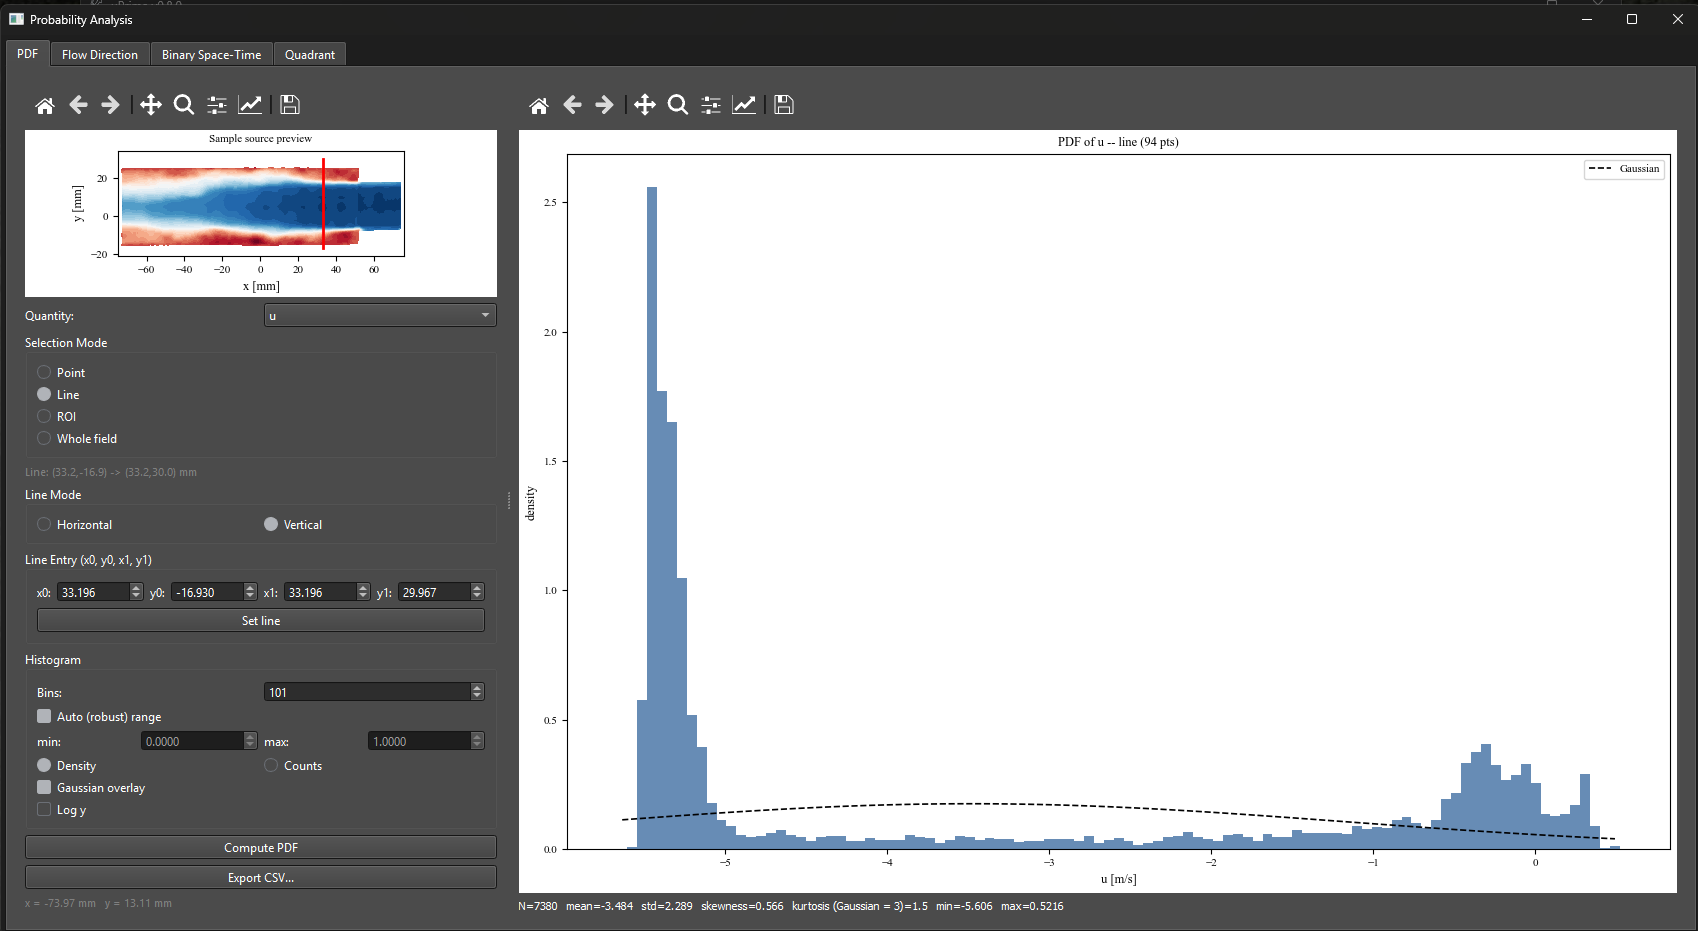
\includegraphics[width=0.98\linewidth]{fig_prob_pdf}
  \caption{Probability Analysis window, `PDF` tab. A vertical sampling line at $x = 33.2$\,mm (red, in the sample-source preview at the top left) pools 94 grid points over all snapshots into a single distribution of the streamwise velocity $u$, giving $N = 7380$ valid samples. The distribution is clearly bimodal, with a sharp peak near $u \approx -5.4$\,m/s and a broad secondary peak near $u \approx 0$: the line crosses two distinct flow regions. The dashed Gaussian overlay, built from the same mean ($-3.484$\,m/s) and standard deviation ($2.289$\,m/s), fails to describe either peak. The kurtosis of 1.5, well below the Gaussian value of 3, is the quantitative signature of that bimodality, and is exactly the information a Reynolds stress map cannot show.}
  \label{fig:prob_pdf}
\end{figure}

\begin{quote}
\textbf{Tip:}
Compare a point PDF inside a shear layer with one in the free stream. The free-stream distribution is close to Gaussian ($S \approx 0$, $F \approx 3$); the shear-layer distribution is typically skewed and has a flatness well above 3. That difference is invisible in the Reynolds stress map, which reports only $\langle q'^2 \rangle$.
\end{quote}

\begin{quote}
\textbf{Warning:}
A converged mean does not imply a converged PDF. The tails of the distribution are governed by the rarest events, so the fourth moment needs far more snapshots than the second. Treat $F$ from a few hundred snapshots as indicative only, and verify convergence in the `Mean \& Convergence` module (Chapter~\ref{ch:meanconv}) first.
\end{quote}

\subsection{Flow Direction tab}

For each grid point, the fraction of snapshots in which the streamwise velocity is positive defines the \textbf{forward-flow probability}
\[
\mathrm{FFP}(x,y) = \frac{1}{N_{\mathrm{valid}}(x,y)} \sum_{n=1}^{N_t} \mathcal{H}\!\left[u_n(x,y)\right],
\qquad
\mathrm{RFP}(x,y) = 1 - \mathrm{FFP}(x,y),
\]
where $\mathcal{H}$ is the Heaviside step function and $N_{\mathrm{valid}}$ is the number of valid (non-NaN) snapshots at that point. RFP is the \textbf{reverse-flow probability}, identical to the backflow coefficient $\gamma_p$ of Simpson (1989).

This quantity is the standard instantaneous criterion for separation, and it is far more informative than the mean velocity field. Mean separation ($\langle u \rangle = 0$) is a single contour line; the RFP field shows the whole intermittent region in which the flow reverses part of the time. Simpson's widely used states of detachment are defined directly on it:

\begin{table}[htbp]
\centering
\caption{States of turbulent boundary-layer detachment after Simpson (1989), expressed in terms of the reverse-flow probability.}
\begin{tabular}{lll}
\toprule
\textbf{State} & \textbf{Abbreviation} & \textbf{Criterion} \\
\midrule
Incipient detachment            & ID  & $\mathrm{RFP} = 0.01$ \\
Intermittent transitory detachment & ITD & $\mathrm{RFP} = 0.20$ \\
Transitory detachment           & TD  & $\mathrm{RFP} = 0.50$ \\
Detachment (mean separation)    & D   & $\langle \tau_w \rangle = 0$ \\
\bottomrule
\end{tabular}
\end{table}

\noindent\textbf{Reference:} Simpson, R.L. (1989). Turbulent boundary-layer separation. \textit{Annual Review of Fluid Mechanics}, 21, 205--234.

\subsubsection*{Sampling modes}

Flow Direction offers \textbf{ROI} and \textbf{whole domain} only. Line profiles are not offered: FFP and RFP are inherently two-dimensional maps, and a line extracted from a probability field is better produced by exporting the map and sampling it, than by a mode that invites reading a probability along an arbitrary cut as if it were a profile.

When an ROI is set, the computation itself is restricted to the ROI, not merely the display. Grid points outside the ROI are rendered in a distinct neutral grey so that an untouched region is never confused with a region where the probability happens to be low.

\begin{quote}
\textbf{Tip:}
The $\mathrm{RFP} = 0.5$ contour and the mean $\langle u \rangle = 0$ contour usually do not coincide. Plotting both is a quick check on whether your separation region is steady or flapping: a large gap between them means the separation point is moving substantially in time.
\end{quote}

\subsection{Binary Space-Time tab}

\begin{quote}
\textbf{Note:}
This tab requires time-resolved data. Set `Acquisition Type` to TR with a valid $f_s$ in the info ribbon before opening the window, otherwise the tab is disabled.
\end{quote}

A binary space-time map reduces the fluctuation field along a line to its sign alone:
\[
b(s, t) = \operatorname{sign}\!\left[q'(s, t)\right] \in \{-1, +1\},
\]
where $s$ is the distance along the selected line and $t$ is time. The result is plotted as a two-colour map with $t$ on the horizontal axis and $s$ on the vertical axis. Amplitude information is deliberately discarded; what remains is the topology of the fluctuation field, which is exactly what is needed to see coherent structures.

Three features are read directly from such a map:

\begin{itemize}[leftmargin=1.5em]
  \item \textbf{Inclination}: coherent structures convecting past the line produce slanted stripes. The slope $\mathrm{d}s/\mathrm{d}t$ of a stripe is a convection velocity, which can be compared against the local mean velocity to test Taylor's hypothesis.
  \item \textbf{Streamwise extent}: the horizontal width of a stripe, multiplied by the convection velocity, estimates the structure length. This is a direct, geometric alternative to the integral scale from the two-point correlation (Chapter~\ref{ch:correlation}).
  \item \textbf{Persistence}: how long a single sign survives before flipping, which characterises the lifetime of the structure at that location.
\end{itemize}

Only horizontal and vertical lines are offered. The map's vertical axis must be a physical distance with uniform spacing for the stripe slopes to be interpretable as velocities, which an interpolated oblique line does not guarantee.

\noindent\textbf{References:} del \'Alamo, J.C. \& Jim\'enez, J. (2009). Estimation of turbulent convection velocities and corrections to Taylor's approximation. \textit{Journal of Fluid Mechanics}, 640, 5--26. Dennis, D.J.C. \& Nickels, T.B. (2011). Experimental measurement of large-scale three-dimensional structures in a turbulent boundary layer. \textit{Journal of Fluid Mechanics}, 673, 180--217.

\subsection{Quadrant tab}

Quadrant analysis asks which kinds of motion produce the Reynolds shear stress $\langle u'v' \rangle$. Each instantaneous sample is classified by the signs of $u'$ and $v'$ into one of four quadrants of the $(u', v')$ plane. The `Pair` selector chooses which two fluctuation components define the plane; $u'$--$v'$ is the standard choice and the only one for which the quadrant names below apply, the other pairs being available for stereo data.

\begin{table}[htbp]
\centering
\caption{Quadrant classification of the instantaneous Reynolds shear stress.}
\begin{tabular}{llll}
\toprule
\textbf{Quadrant} & \textbf{Signs} & \textbf{Name} & \textbf{Contribution to $\langle u'v' \rangle$} \\
\midrule
Q1 & $u' > 0$, $v' > 0$ & Outward interaction & Positive \\
Q2 & $u' < 0$, $v' > 0$ & Ejection            & Negative \\
Q3 & $u' < 0$, $v' < 0$ & Inward interaction  & Positive \\
Q4 & $u' > 0$, $v' < 0$ & Sweep               & Negative \\
\bottomrule
\end{tabular}
\end{table}

In a wall-bounded shear flow with $\mathrm{d}\langle u \rangle/\mathrm{d}y > 0$, the shear stress $\langle u'v' \rangle$ is negative and is generated almost entirely by Q2 and Q4: low-momentum fluid lifted away from the wall (ejections) and high-momentum fluid swept toward it (sweeps). Q1 and Q3 oppose the mean transport and typically contribute far less. The near-wall balance between ejections and sweeps is one of the most-used descriptors of wall turbulence.

Two fractions are reported per quadrant $i$:
\[
T_i = \frac{N_i}{N_{\mathrm{valid}}}
\qquad\text{(time fraction)},
\qquad
S_i = \frac{\langle u'v' \rangle_i}{\langle u'v' \rangle}
\qquad\text{(stress fraction)},
\]
where $\langle u'v' \rangle_i$ is the conditional average taken over the samples in quadrant $i$ only, with the sum over all four quadrants recovering the total. At hole size $H = 0$ the time fractions sum to unity and the stress fractions sum to unity by construction; at $H > 0$ both sums fall below unity, because the excluded weak events are missing by design, and the shortfall itself measures how much of the signal is weak. Note the sign convention: $S_i$ is normalised by $\langle u'v' \rangle$, which is itself negative in a wall-bounded shear flow, so the stress-producing quadrants Q2 and Q4 appear as \emph{positive} fractions and the counter-gradient quadrants Q1 and Q3 as negative ones. Comparing $T_i$ with $S_i$ is the point of the exercise: a quadrant that occupies a small fraction of the time while carrying a large fraction of the stress is by definition intermittent and energetic.

\subsubsection*{Hole size}

To isolate the strongest events, a hole of size $H$ is defined in the $(u', v')$ plane and only samples outside it are counted:
\[
\left| u'v' \right| > H \, u_{\mathrm{rms}} \, v_{\mathrm{rms}} .
\]
$H = 0$ recovers the plain quadrant decomposition with every sample included. Increasing $H$ progressively excludes weak fluctuations near the origin and retains only extreme events. The tab provides both a single-$H$ view and a \textbf{hole-size sweep}, which plots $S_i(H)$ for the four quadrants against $H$. In wall turbulence the Q2 and Q4 curves persist to large $H$ while Q1 and Q3 decay quickly, quantifying how much of the stress is carried by rare, strong events.

A joint PDF of $(u', v')$ is also available, with the quadrant boundaries and the hyperbolic hole contours overlaid, giving the same information in a continuous form. It is drawn on a $\log_{10}(N+1)$ scale, so that the sparsely populated extreme events remain visible next to the dense core.

\subsubsection*{Sampling and outputs}

Sampling is `ROI` or `Whole field`; draw an ROI by right-clicking and dragging on the selection preview. The region applies to the joint histogram and the hole-size sweep only. The two-dimensional stress-fraction maps always use the full domain, since their purpose is to show where in the flow each quadrant dominates.

Clicking `Compute` produces the joint PDF, the quadrant-contribution bar chart, and the Q2 and Q4 stress-fraction maps at the current hole size. `Hole sweep (Lu \& Willmarth)` repeats the decomposition over a range of $H$ and plots the resulting curves. Three separate exports are provided: `Export fractions CSV\ldots` for the per-quadrant numbers, `Export 2D\ldots` for the stress-fraction maps, and `Export hole sweep CSV\ldots` for the sweep curves.

\begin{figure}[htbp]
  \centering
  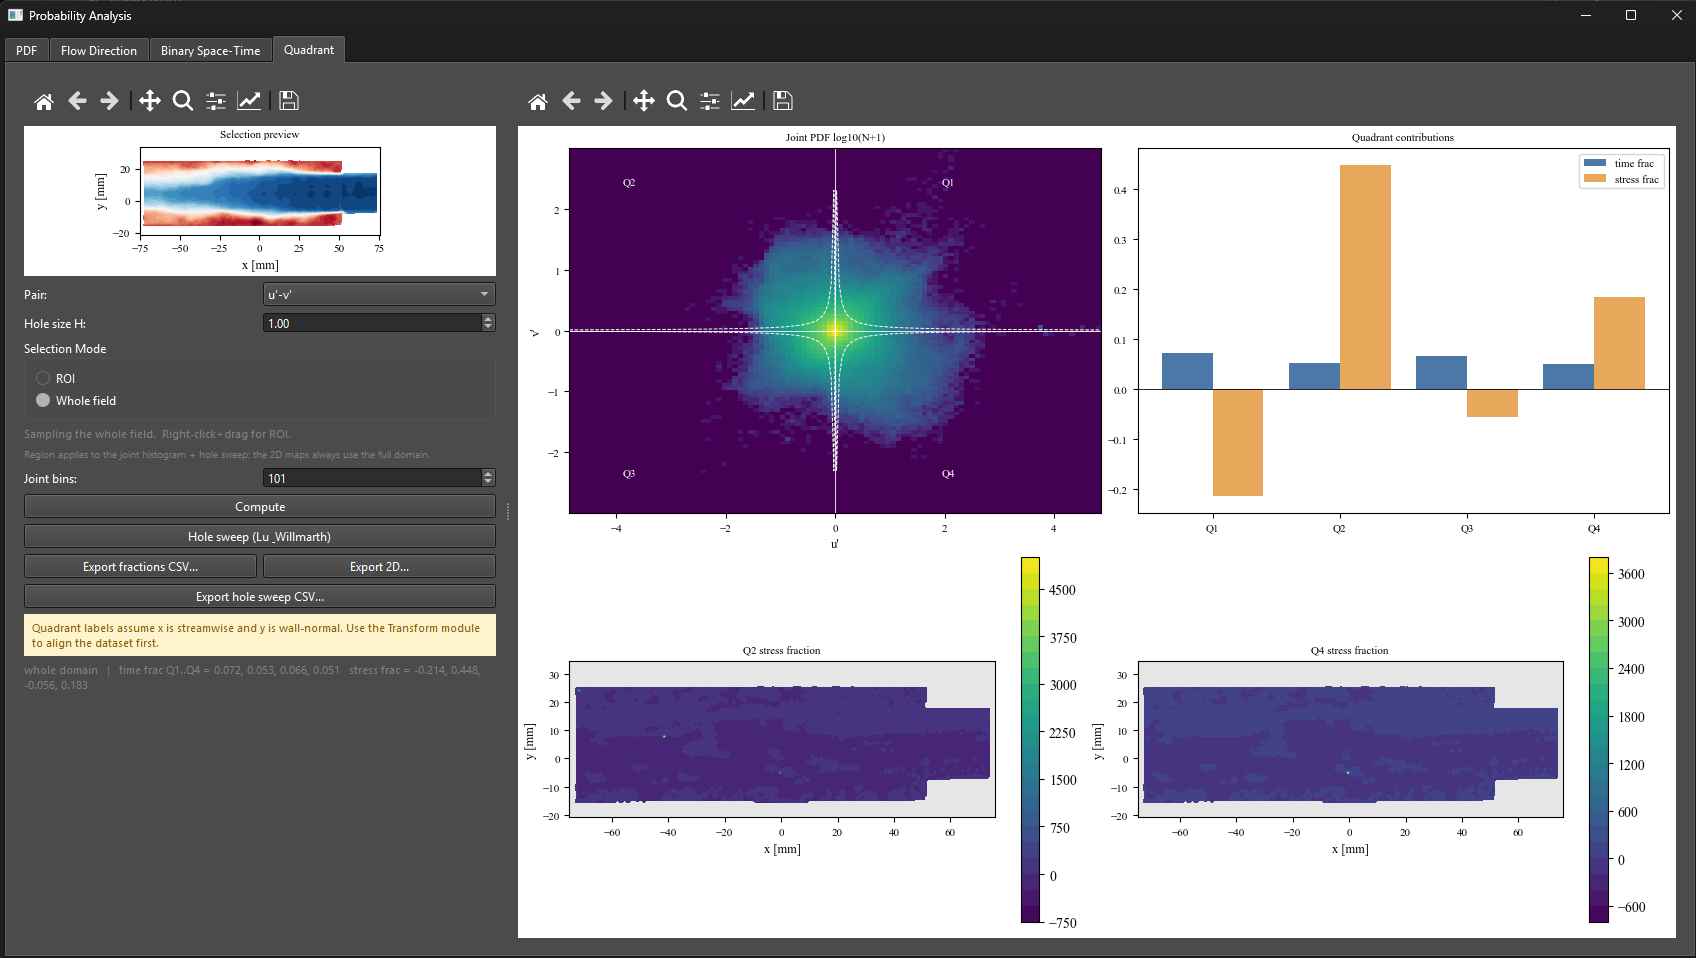
\includegraphics[width=0.98\linewidth]{fig_prob_quadrant}
  \caption{Probability Analysis window, `Quadrant` tab, whole-field sampling at hole size $H = 1$. Top left: joint PDF of $(u', v')$ on a $\log_{10}(N+1)$ scale, with the quadrant boundaries and the hyperbolic hole contours overlaid; only samples outside the hole are counted. Top right: time fractions (blue) and stress fractions (orange) per quadrant. Q2 (ejections, $S_2 = 0.448$) and Q4 (sweeps, $S_4 = 0.183$) carry the stress while Q1 and Q3 oppose it ($-0.214$ and $-0.056$), the classical wall-turbulence balance. Each quadrant occupies only 5 to 7\,\% of the time, and the four time fractions sum to 0.24 rather than 1 because $H = 1$ excludes the weak events. Bottom: Q2 and Q4 stress-fraction maps over the full domain, with masked and invalid regions in grey.}
  \label{fig:prob_quadrant}
\end{figure}

\noindent\textbf{References:} Wallace, J.M., Eckelmann, H. \& Brodkey, R.S. (1972). The wall region in turbulent shear flow. \textit{Journal of Fluid Mechanics}, 54(1), 39--48. Lu, S.S. \& Willmarth, W.W. (1973). Measurements of the structure of the Reynolds stress in a turbulent boundary layer. \textit{Journal of Fluid Mechanics}, 60(3), 481--511. Wallace, J.M. (2016). Quadrant analysis in turbulence research: history and evolution. \textit{Annual Review of Fluid Mechanics}, 48, 131--158.

\begin{quote}
\textbf{Warning:}
Quadrant analysis is defined with respect to the mean shear direction. If the coordinate system is not aligned with the flow, the quadrant labels lose their physical meaning: what the software calls an ejection is then some mixture of ejections and sweeps. Align the dataset in the `Coordinate Transform` module (Chapter~\ref{ch:transform}) before running this tab.
\end{quote}

\subsection{Exporting}

Every tab exports through the standard \href{https://cmdrryder.github.io/uPrime/}{uPrime} paths. One-dimensional results (PDF histograms, hole-size sweeps, quadrant fractions) export as \texttt{.csv} with a full settings header block recording the quantity, sampling mode, sampling geometry, bin count, hole size, and valid-sample count. Two-dimensional results (FFP/RFP maps, joint PDFs, binary space-time maps) export as Tecplot \texttt{.dat} through the shared 2D writer, and as PNG (300\,DPI), PDF, or SVG figures from the toolbar. Exported CSV profiles can be re-imported into the `Compare Cases` viewer (Chapter~\ref{ch:comparecases}) to overlay probability results from different runs.

% ============================= CHAPTER 14 ==============================
